\begin{figure}
	\centering
	\subfigure[Sol]{
	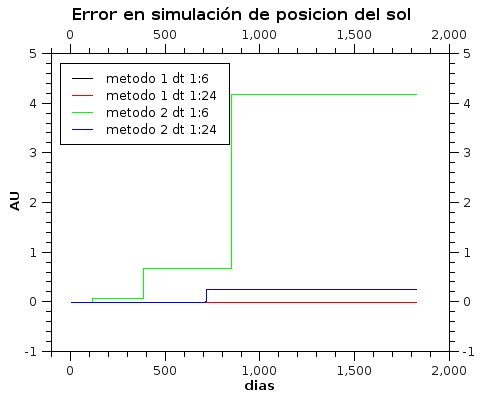
\includegraphics[scale=0.5]{img/ej1/error/error_sol.png}
	\label{fig:ej1_err_sol_4}
	}
	\subfigure[Tierra]{
	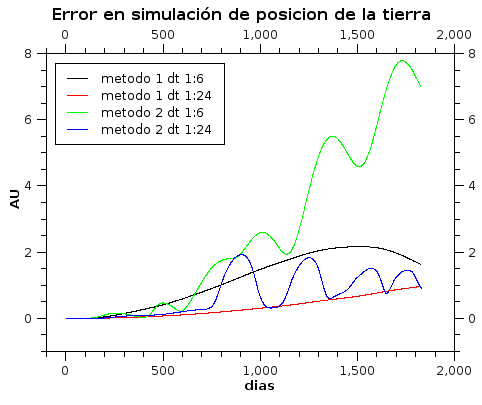
\includegraphics[scale=0.5]{img/ej1/error/error_tierra.png}
	\label{fig:ej1_err_sol_24}
	}
	\\
	\subfigure[Luna]{
	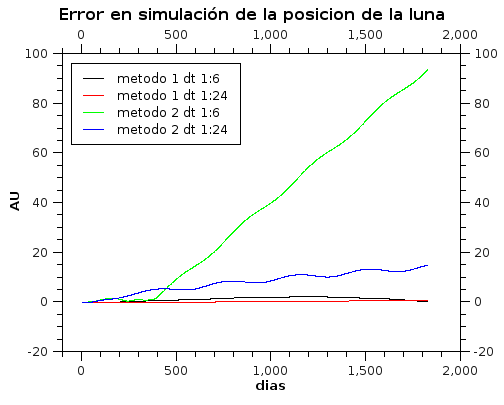
\includegraphics[scale=0.5]{img/ej1/error/error_luna.png}
	\label{fig:ej1_err_tierra_4}
	}
	\caption{
		Errores de las posiciónes simuladas de los cuerpos sol, tierra y luna,
		con respecto a los datos de la NASA en función del tiempo.
		El error fua calculado como la norma entre la diferencia de los
		vectores de posición de la NASA y los simulados por nosotros.
		El período de simulación es de 5 años.
	}
	\label{ fig:res_ej1_err }
\end{figure}
